\documentclass[12pt]{article}
\usepackage{graphicx} % Required for inserting images
\usepackage[greek,english]{babel}
\usepackage{xgreek}

% FONTS
% \usepackage{xunicode}
\usepackage{xltxtra}
% \defaultfontfeatures{Mapping=tex-text} % converts LaTeX specials (``quotes'' --- dashes etc.) to unicode
% \setromanfont [Ligatures={Common}, BoldFont={GFS Artemisia Bold}, ItalicFont={Gentium Italic}]{Gentium}
% \setmonofont[Scale=0.8]{GFS Artemisia} 
\setmainfont{GFS Artemisia}

\usepackage{geometry} 
\geometry{a4paper, textwidth=5.5in, textheight=8.5in, marginparsep=7pt, marginparwidth=.6in}
\setlength\parindent{8mm}
\setlength\parskip{5mm}

% \usepackage{unicode-math}
\usepackage[shortlabels]{enumitem}

% diagram support
\usepackage{tikz}
\usetikzlibrary{arrows,calc,patterns,positioning,shapes}
\usetikzlibrary{decorations.pathmorphing}

\tikzset{
modal/.style={>=stealth',shorten >=1pt,shorten <=1pt,auto,
    node distance=1.5cm,thick},
world/.style={circle,draw,minimum size=1cm,fill=gray!15},
point/.style={circle,draw,fill=black,inner sep=0.5mm},
reflexive/.style={->,in=120,out=60,loop,looseness=#1},
reflexive/.default={5},
reflexive point/.style={->,in=135,out=45,loop,looseness=#1},
reflexive point/.default={25},
}
\tikzset{
reflexive above/.style={->,loop,in=120,out=60,looseness=#1},
reflexive above/.default={7},
reflexive below/.style={->,loop,in=240,out=300,looseness=#1},
reflexive below/.default={7},
reflexive left/.style={->,loop,in=150,out=210,looseness=#1},
reflexive left/.default={7},
reflexive right/.style={->,loop,in=30,out=330,looseness=#1},
reflexive right/.default={7}
}

\title{Άσκηση 1.3 από \\``Reasoning About Knowledge (1995)''}
\author{Καμινάρης Κωνσταντίνος}
\date{11/3/2024}

%%%%%%%%% END OF PREAMBLE %%%%%%%%%%%%

\begin{document}

\setlanguage{greek} %% this is to activate greek hyphenation

\maketitle

\section*{Άσκηση 1.3}
\subsection*{Ερώτηση}
The wise men puzzle is a well-known variant of the muddy children puzzle.
The standard version of the story goes as follows: There are three wise men. It is
common knowledge that there are three red hats and two white hats. The king puts
a hat on the head of each of the three wise men, and asks them (sequentially) if they
know the color of the hat on their head. The first wise man says that he does not
know; the second wise man says that he does not know; then the third wise man says
that he knows.

\begin{enumerate}[label=\emph{\alph*}]
    \item What color is the third wise man’s hat?
    \item We have implicitly assumed in the story that the wise men can all see. Suppose we assume instead that the third wise man is blind and that it is common knowledge that the first two wise men can see. Can the third wise man still figure out the color of his hat?
\end{enumerate}

\newpage

\subsection*{Απάντηση για ταυτόχρονες αποκρίσεις}

Στην ανάλυση που ακολουθεί έχει γίνει η σημαντική παραδοχή πως οι απαντήσεις των παικτών είναι ταυτόχρονες (και όχι με τη σειρά). Επίσης έχει γίνει η (λιγότερο σημαντική) παραδοχή πως τα καπέλα είναι 3 λευκά και 2 μαύρα αντί για τα 3 κόκκινα και 2 λευκά της εκφώνησης. Θα χρησιμοποιηθούν οι ατομικές προτάσεις $AisWh$, $BisWh$ και $CisWh$, με την ευκόλως εννοούμενη ερμηνεία τους.

\begin{table}[h!]
\centering
\begin{tabular}{ c|c c c }
  & A & B & C \\
 \hline
 s1 & W & W & W \\ 
 \hline
 s2 & B & W & W \\
 \hline
 s3 & W & B & W \\ 
 \hline
 s4 & W & W & B \\ 
 \hline
 s5 & B & B & W \\ 
 \hline
 s6 & B & W & B \\ 
 \hline
 s7 & W & B & B \\ 
\end{tabular}
\caption{Πιθανοί κόσμοι}
\label{worlds}
\end{table}

\begin{figure}[h!]
\centering
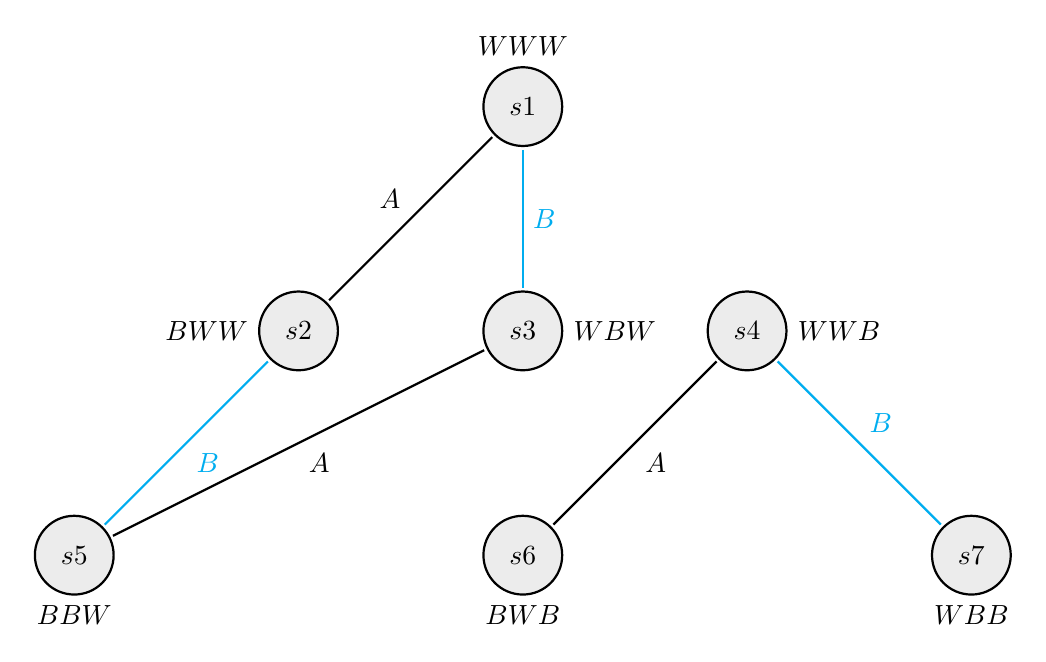
\begin{tikzpicture}[modal, node distance=3cm]

    \node[world] (1) [label=above:$W W W$] {$s1$};
    \node[world] (2) [label=left:$B W W$,below left=of 1] {$s2$};
    \node[world] (3) [label=right:$W B W$] at (2 -| 1) {$s3$};
    \node[world] (4) [label=right:$W W B$,below right=of 1] {$s4$};
    \node[world] (5) [label=below:$B B W$,below left=of 2] {$s5$};
    \node[world] (6) [label=below:$B W B$] at (5 -| 3) {$s6$};
    \node[world] (7) [label=below:$W B B$,below right=of 4] {$s7$};
    
    \path[-]
        (1) edge[color=cyan] node[] {$B$} (3)
        (2) edge[] node[] {$A$} (1)
            edge[color=cyan] node[] {$B$} (5)
        (3) edge[] node[] {$A$} (5)
        (4) edge[] node[] {$A$} (6)
            edge[color=cyan] node[] {$B$} (7)
    ;        
\end{tikzpicture}
\caption{M1}
\label{M1}
\end{figure}

Θα ασχοληθούμε με το ερώτημα β'. Η λίστα με όλους τους πιθανούς κόσμους φαίνεται στον πίνακα \ref{worlds}. Το αντίστοιχο διάγραμμα Kripke φαίνεται στο σχήμα \ref{M1}. Εφόσον είναι κοινή γνώση πως ο παίκτης C είναι τυφλός, όλοι οι πιθανοί κόσμοι είναι ισοδύναμοι για τον παίκτη C. Επομένως υπάρχουν ακμές για τον C από κάθε κόσμο σε κάθε άλλο κόσμο. Οι ακμές αυτές δεν αναπαρίστανται για λόγους ευκρίνειας. Παρατηρούμε πως $(K_A\ AisWh)$ αληθεύει μόνο στην κατάσταση $s7$, ενώ $(K_B\ BisWh)$ ισχύει μόνο στην κατάσταση $s6$.

Θα διακρίνουμε τώρα δύο περιπτώσεις. Αν στην πρώτη ερώτηση του βασιλιά είτε ο A, είτε ο B απαντήσουν πως ξέρουν το χρώμα του καπέλου τους, τότε βρισκόμαστε είτε στην κατάσταση $s7$, είτε στην κατάσταση $s6$ αντίστοιχα. Παρατηρούμε τώρα πως ο παίκτης C έχει μαύρο καπέλο και στις δύο αυτές καταστάσεις. Άρα όλοι οι παίκτες ξέρουν το χρώμα τους μετά τη δεύτερη ερώτηση του βασιλιά. Αντιθέτως αν όλοι απαντήσουν αρνητικά στην πρώτη ερώτηση, τότε το διάγραμμα Kripke αλλάζει όπως φαίνεται στο σχήμα \ref{M2} (Οι ακμές του παίκτη C παραλείπονται για λόγους ευκρίνειας).

\begin{figure}[h!]
\centering
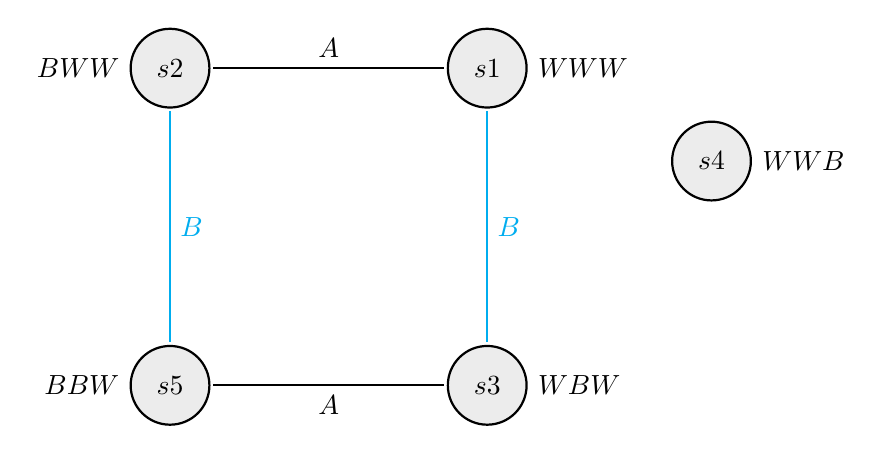
\begin{tikzpicture}[modal, node distance=3cm]

    \node[world] (1) [label=right:$W W W$] {$s1$};
    \node[world] (2) [label=left:$B W W$,left=of 1] {$s2$};
    \node[world] (3) [label=right:$W B W$,below=of 1] {$s3$};
    \node[world] (4) [label=right:$W W B$,above right=of 3] {$s4$};
    \node[world] (5) [label=left:$B B W$,below=of 2] {$s5$};
    
    \path[-]
        (1) edge[color=cyan] node[] {$B$} (3)
        (2) edge[] node[] {$A$} (1)
            edge[color=cyan] node[] {$B$} (5)
        (3) edge[] node[] {$A$} (5)
    ;        
\end{tikzpicture}
\caption{M2}
\label{M2}
\end{figure}

Παρατηρούμε τώρα ότι $(K_A\ AisWh \land K_B\ BisWh)$ αληθεύει μόνο στην κατάσταση $s4$. Θα διακρίνουμε όπως πριν δύο περιπτώσεις. Αν στη δεύτερη ερώτηση ο A και ο B απαντήσουν θετικά, τότε ο παίκτης C μαθαίνει πως φοράει μαύρο καπέλο και μπορεί να απαντήσει θετικά στην τρίτη ερώτηση. Αντιθέτως αν όλοι απαντήσουν αρνητικά στη δεύτερη ερώτηση, τότε το διάγραμμα Kripke αλλάζει όπως φαίνεται στο σχήμα \ref{M3}. Παρατηρούμε όμως πως $(CisWh)$ αληθεύει σε όλες τις πιθανές καταστάσεις του διαγράμματος, κι έτσι ο παίκτης C θα απαντήσει θετικά στην τρίτη ερώτηση. Ταυτόχρονα όμως, επειδή $(CisWh)$ αληθεύει σε όλες τις πιθανές καταστάσεις, ισχύει ότι $(C\ CisWh)$. Σε αυτή την περίπτωση οι παίκτες A και B δε θα μάθουν ποτέ το χρώμα του καπέλου τους, όσες φορές κι αν ρωτήσει ο βασιλιάς. Το διάγραμμα Kripke μένει στάσιμο από εδώ και στο εξής γιατί κανένας παίκτης δεν αποκτά καινούργια πληροφορία.

\begin{figure}[h!]
\centering
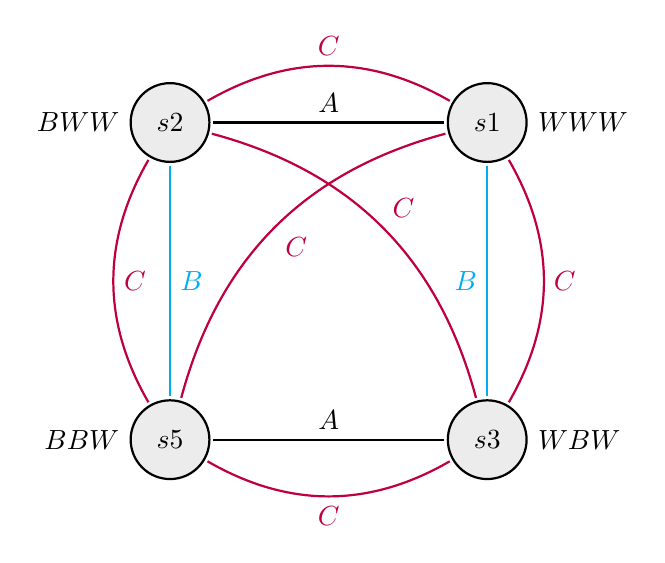
\begin{tikzpicture}[modal, node distance=3cm]

    \node[world] (1) [label=right:$W W W$] {$s1$};
    \node[world] (2) [label=left:$B W W$,left=of 1] {$s2$};
    \node[world] (3) [label=right:$W B W$,below=of 1] {$s3$};
    \node[world] (5) [label=left:$B B W$,below=of 2] {$s5$};
    
    \path[-]
        (1) edge[color=cyan] node[left] {$B$} (3)
            edge[bend left, color=purple] node[] {$C$} (3)
            edge[bend right, color=purple] node[] {$C$} (5)
        (2) edge[] node[] {$A$} (1)
            edge[color=cyan] node[] {$B$} (5)
            edge[bend left, color=purple] node[] {$C$} (1)
            edge[bend left, color=purple] node[] {$C$} (3)
            edge[bend right, color=purple] node[] {$C$} (5)
        (3) edge[] node[above] {$A$} (5)
            edge[bend left, color=purple] node[] {$C$} (5)
    ;        
\end{tikzpicture}
\caption{M3}
\label{M3}
\end{figure}

\subsection*{Απάντηση για διαδοχικές αποκρίσεις}

Στην περίπτωση που οι παίκτες αποκρίνονται διαδοχικά το αρχικό διάγραμμα Kripke είναι ξανά το σχήμα \ref{M1}. Παρατηρούμε, όπως και προηγουμένως, πως $(K_A\ AisWh)$ αληθεύει μόνο στην κατάσταση $s7$, ενώ $(K_B\ BisWh)$ ισχύει μόνο στην κατάσταση $s6$. Αν ο παίκτης A απαντήσει θετικά, τότε όλοι οι παίκτες ξέρουν πως βρισκόμαστε στην κατάσταση $s7$, και άρα όλοι μαθαίνουν το χρώμα τους. Αντιθέτως, αν ο παίκτης A απαντήσει αρνητικά, τότε το διάγραμμα Kripke αλλάζει όπως φαίνεται στο σχήμα \ref{M4} (Οι ακμές του παίκτη C παραλείπονται για λόγους ευκρίνειας). 

\begin{figure}[h!]
\centering
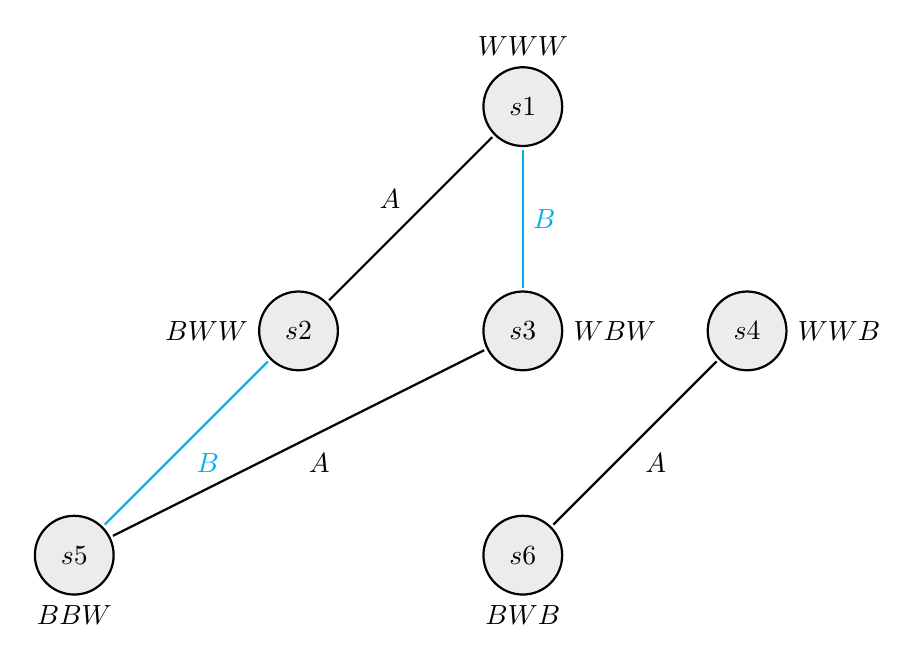
\begin{tikzpicture}[modal, node distance=3cm]

    \node[world] (1) [label=above:$W W W$] {$s1$};
    \node[world] (2) [label=left:$B W W$,below left=of 1] {$s2$};
    \node[world] (3) [label=right:$W B W$] at (2 -| 1) {$s3$};
    \node[world] (4) [label=right:$W W B$,below right=of 1] {$s4$};
    \node[world] (5) [label=below:$B B W$,below left=of 2] {$s5$};
    \node[world] (6) [label=below:$B W B$] at (5 -| 3) {$s6$};
    
    \path[-]
        (1) edge[color=cyan] node[] {$B$} (3)
        (2) edge[] node[] {$A$} (1)
            edge[color=cyan] node[] {$B$} (5)
        (3) edge[] node[] {$A$} (5)
        (4) edge[] node[] {$A$} (6)
    ;        
\end{tikzpicture}
\caption{M4}
\label{M4}
\end{figure}

Παρατηρούμε τώρα ότι $(K_B\ BisWh)$ αληθεύει στις καταστάσεις $s4$ και $s6$. Θα διακρίνουμε δύο περιπτώσεις. Αν ο Β απαντήσει αρνητικά, τότε το διάγραμμα Kripke αλλάζει όπως φαίνεται στο σχήμα \ref{M3}. Όμως, όπως και πριν, $(K_C\ CisWh)$ ισχύει σε όλες τις καταστάσεις του σχήματος \ref{M3}. Έτσι λοιπόν, ο παίκτης C μαθαίνει το χρώμα του και απαντά θετικά.

\begin{figure}[h!]
\centering
\begin{tikzpicture}[modal, node distance=3cm]

    \node[world] (4) [label=right:$W W B$,below right=of 1] {$s4$};
    \node[world] (6) [label=below:$B W B$] at (5 -| 3) {$s6$};
    
    \path[-]
        (4) edge[] node[] {$A$} (6)
        (4) edge[color=purple, bend left] node[] {$C$} (6)
    ;        
\end{tikzpicture}
\caption{M5}
\label{M5}
\end{figure}

Αντιθέτως, αν ο παίκτης B απαντήσει θετικά, τότε το διάγραμμα Kripke αλλάζει όπως φαίνεται στο σχήμα \ref{M5}. Παρατηρούμε ότι $(K_C\ \neg CisWh)$ ισχύει σε όλες τις καταστάσεις του σχήματος \ref{M5}. Έτσι, ο παίκτης C μαθαίνει το χρώμα του και απαντά θετικά. Ο παίκτης Α δεν μαθαίνει κάποια καινούργια πληροφορία μετά την απόκριση του C κι έτσι δε θα μάθει ποτέ το χρώμα του, όσες φορές κι αν ρωτήσει ο βασιλιάς.

\subsection*{Συμπέρασμα}

Συμπερασματικά, στην περίπτωση που είναι κοινή γνώση πως ο παίκτης C είναι τυφλός, τότε το αν αυτός θα μπορέσει να μάθει το χρώμα του εξαρτάται από τον τρόπο που αποκρίνονται οι παίκτες. Πιο συγκεκριμένα, αν οι παίκτες αποκρίνονται διαδοχικά (πρώτα ο A, μετά ο B, μετά ο C), τότε ο παίκτης C θα μπορέσει να απαντήσει θετικά με την πρώτη ερώτηση του βασιλιά. Αν όμως οι παίκτες αποκρίνονται ταυτόχρονα, τότε ο παίκτης C μπορεί να μη μπορέσει να αποκριθεί με την πρώτη ερώτηση του βασιλιά, και να χρειαστεί άλλες δύο ερωτήσεις για να απαντήσει θετικά.

\end{document}
